\documentclass[conference]{IEEEtran}

% *** PDF, URL AND HYPERLINK PACKAGES ***
%
%\usepackage{url}
% url.sty was written by Donald Arseneau. It provides better support for
% handling and breaking URLs. url.sty is already installed on most LaTeX
% systems. The latest version and documentation can be obtained at:
% http://www.ctan.org/pkg/url
% Basically, \url{my_url_here}.

% for figures
\usepackage{graphicx}
\usepackage{hyperref}
\usepackage{array}
\newcolumntype{L}[1]{>{\raggedright\let\newline\\\arraybackslash\hspace{0pt}}m{#1}}
\newcolumntype{C}[1]{>{\centering\let\newline\\\arraybackslash\hspace{0pt}}m{#1}}
\newcolumntype{R}[1]{>{\raggedleft\let\newline\\\arraybackslash\hspace{0pt}}m{#1}}


\begin{document}
%
% paper title
% Titles are generally capitalized except for words such as a, an, and, as,
% at, but, by, for, in, nor, of, on, or, the, to and up, which are usually
% not capitalized unless they are the first or last word of the title.
% Linebreaks \\ can be used within to get better formatting as desired.
% Do not put math or special symbols in the title.
\title{Magic Mirror Web Interface\\ Using the Raspberry PI}

% author names and affiliations
% use a multiple column layout for up to three different
% affiliations
\author{\IEEEauthorblockN{Michael Meding}
\IEEEauthorblockA{University of Massachusetts Lowell\\Computer Science\\
Lowell, Massachusetts 01852\\
Email: mike@mikemeding.com}
\and
\IEEEauthorblockN{Peter Welby}
\IEEEauthorblockA{University of Massachusetts Lowell\\Computer Science\\
Lowell, Massachusetts 01852\\
Email: pwelby@cs.uml.edu}
\and
\IEEEauthorblockN{Harun Guna}
\IEEEauthorblockA{University of Massachusetts Lowell\\Computer Science\\
Lowell, Massachusetts 01852\\
Email: harung1993@gmail.com}
}

% make the title area
\maketitle

% As a general rule, do not put math, special symbols or citations
% in the abstract
\begin{abstract}
This semesters IoT project was building a “Magic Mirror”. 
A Magic Mirror is a piece of 1 way glass with a computer monitor behind it to display a set of dynamic information such as the news, weather, or personal calendar events in the presence of person in front of it.
\end{abstract}


\section{Introduction}
%A brief introduction to the background, motivation of the work, challenges of performing the work, contributions of the work and the structure of the rest of the paper. Novelty of the work should be emphasized in the section of introduction.
A Magic Mirror is a Raspberry Pi powered computer display that sits behind a sheet of one way mirror glass as shown in Figure \ref{fig:mirror}.
The Mirror is designed to detect the presence of person and activate the display when a person is detected.
Displayed on the screen are various dynamic items which the user may find helpful when looking in the mirror such as the current weather and time.
\begin{figure}[!ht]
  \centering
  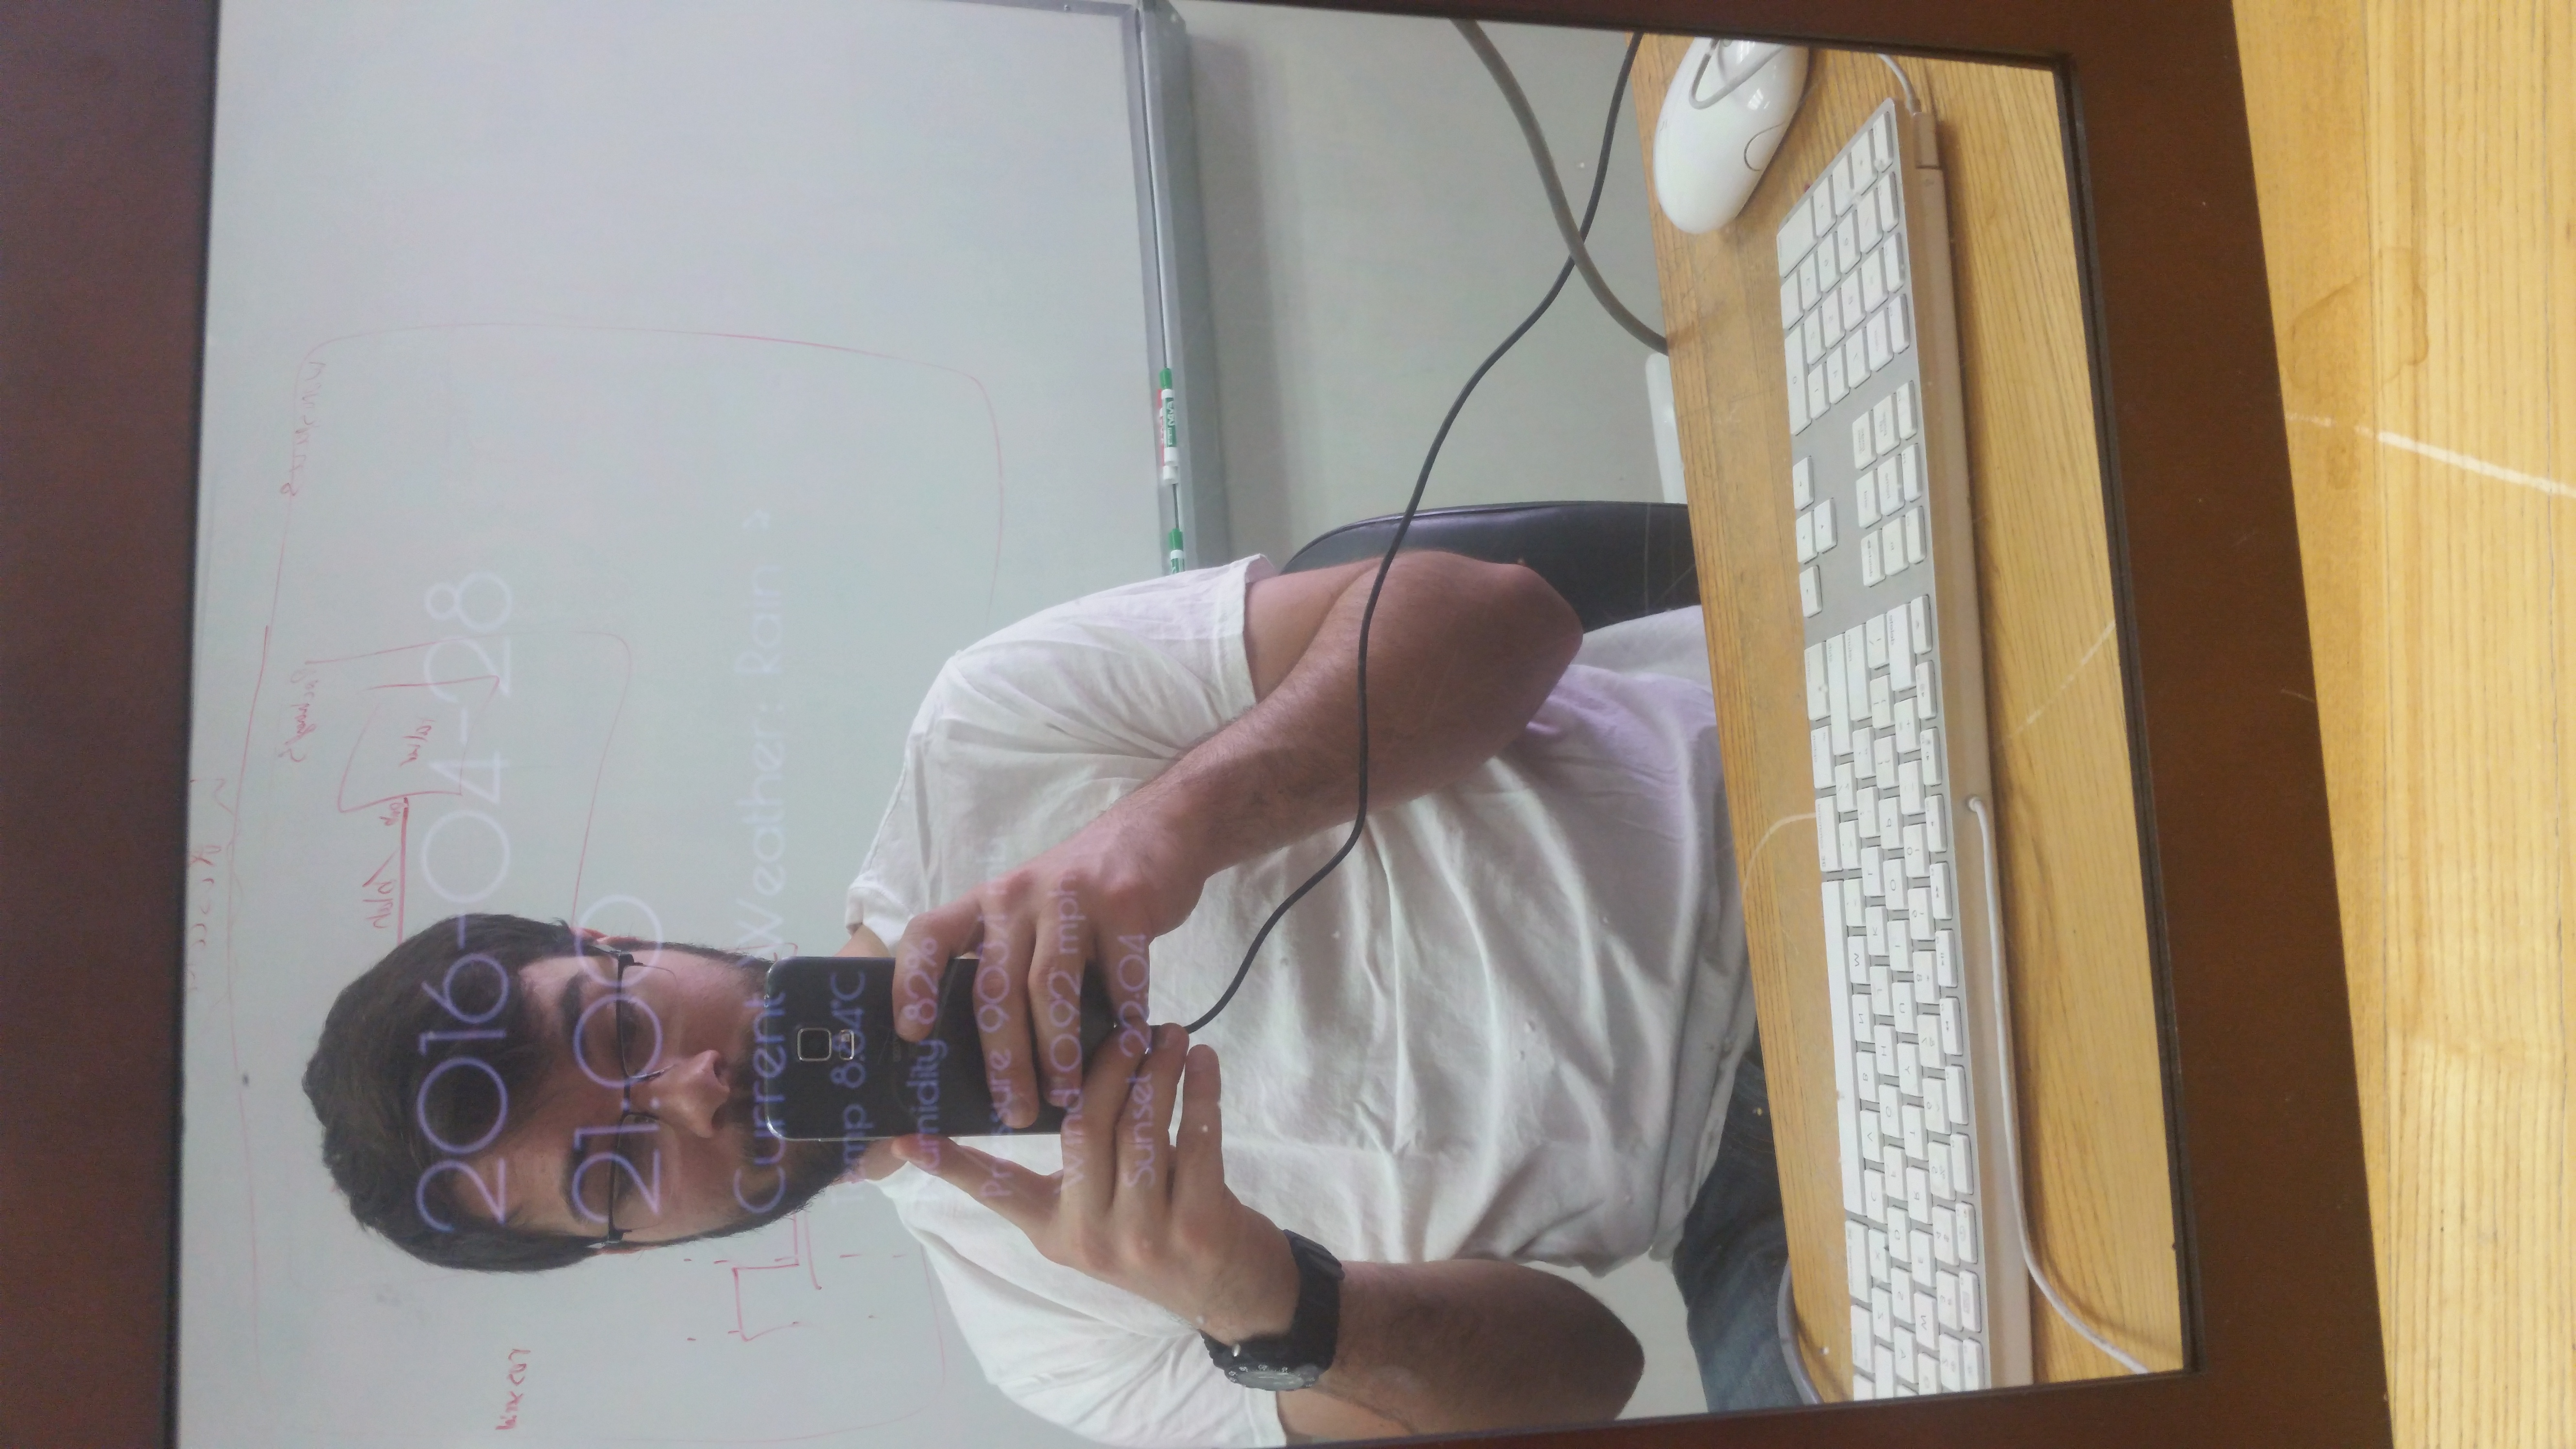
\includegraphics[width=2.5in, angle=-90]{images/Mirror.jpg}
  \caption{The finished Magic Mirror in action. Note the displayed text which appears near the dark regions of the photo.}
  \label{fig:mirror}
\end{figure}


\section{Related Work}  
%An academic paper should demonstrate novelties, i.e., things and/or theories that have not been done in the whole world. This requires the authors to be familiar with the complete bibliography. The most related work to this paper should be presented in this section. Comparison should be made whenever necessary to demonstrate the difference between this work and related work.
%REMEMBER TO CITE!!!!


%%% Harun, you need to find the original project that this is based on and cite it.
%%% also talk about how our project differs from that original project.
This project was inspired by the already existing work of \href{michaelteeuw.nl}{ Michael Teeuw } . The hardware implementation we followed is straighforward follows the work of  \href{http://michaelteeuw.nl/post/80391333672/magic-mirror-part-i-the-idea-the-mirror}{Michael Teeuw's Step by Step guide}. As we went along with the implementation we came across an idea of including a PIR sensor. By employing PIR we can detect the human presence , thereby automating the screen to turn on and off when someone stands infront of it. This not only provides a futuristic feature but also conserves energy . 


\section{System} 
%The name of this section can be the name of the actual system students are developing or other meaningful names. A detailed description of the system. The overall design of the system should be presented first, followed by detailed introduction to complicated components. Subsections should be used whenever necessary, for example, when the content is too long as one section/subsection.
Building the Magic Mirror consisted of two parts, building the device, and writing an intuitive web interface.
\subsection{Building the Magic Mirror}
The mirror that was constructed for this project was assembled using a variety of used electronics as shown by the cost breakdown in Table \ref{tab:cost}.
Dimensions of the mirror when finished were 11x17 for the mirror size and then slightly larger than that including the width of the frame.
The build process took about 3 weeks from start to finish and the most difficult portion of the build was getting all the electronics to work together.
An LCD television was the base platform which drove all the other design choices such as how large to cut the frame how to power the Raspberry PI.
The glass of mirror consisted of a sheet of 1/8 inch Plexiglas covered in automotive 1 way window tint.
This window tint is what gives the mirror the holographic effect when high contrast text is shown on the display.

\begin{table}[!t]
% increase table row spacing, adjust to taste
\renewcommand{\arraystretch}{1.3}
\caption{Parts List and Cost}
\label{tab:cost}
\centering
% Some packages, such as MDW tools, offer better commands for making tables
% than the plain LaTeX2e tabular which is used here.
\begin{tabular}{|l|c|}
\hline
Part Description & Cost\\
\hline
\hline
Raspberry PI & \$35\\
\hline
PIR Sensor & \$15\\
\hline
Small LCD Television & Free*\\
\hline
USB Wireless Card & \$5\\
\hline
Automotive Window Tint & \$10\\
\hline
Plexiglas & \$7\\
\hline
Used Picture Frame & \$5\\
\hline
Misc. Fasteners & \$10\\
\hline
\hline
Total & \$87\\
\hline
\end{tabular}
\end{table}

\subsection{Programming the Magic Mirror}
Programming the Magic Mirror required setting up a web-based Python environment.
For this Django was chosen as it is one of the best supported environments for server side python.
This made the integration with AWS IoT simple as many of the examples online are shown in python.
In addition to sending status messages to AWS IoT the Magic Mirror also has its own local database where it stores its settings.
These settings are unique to the device and consist of custom messages that the user has made and the current location settings of the device.
A breakdown of the structure of the Magic Mirror software is shown in Figure \ref{fig:design}.

\begin{figure}[!ht]
  \centering
  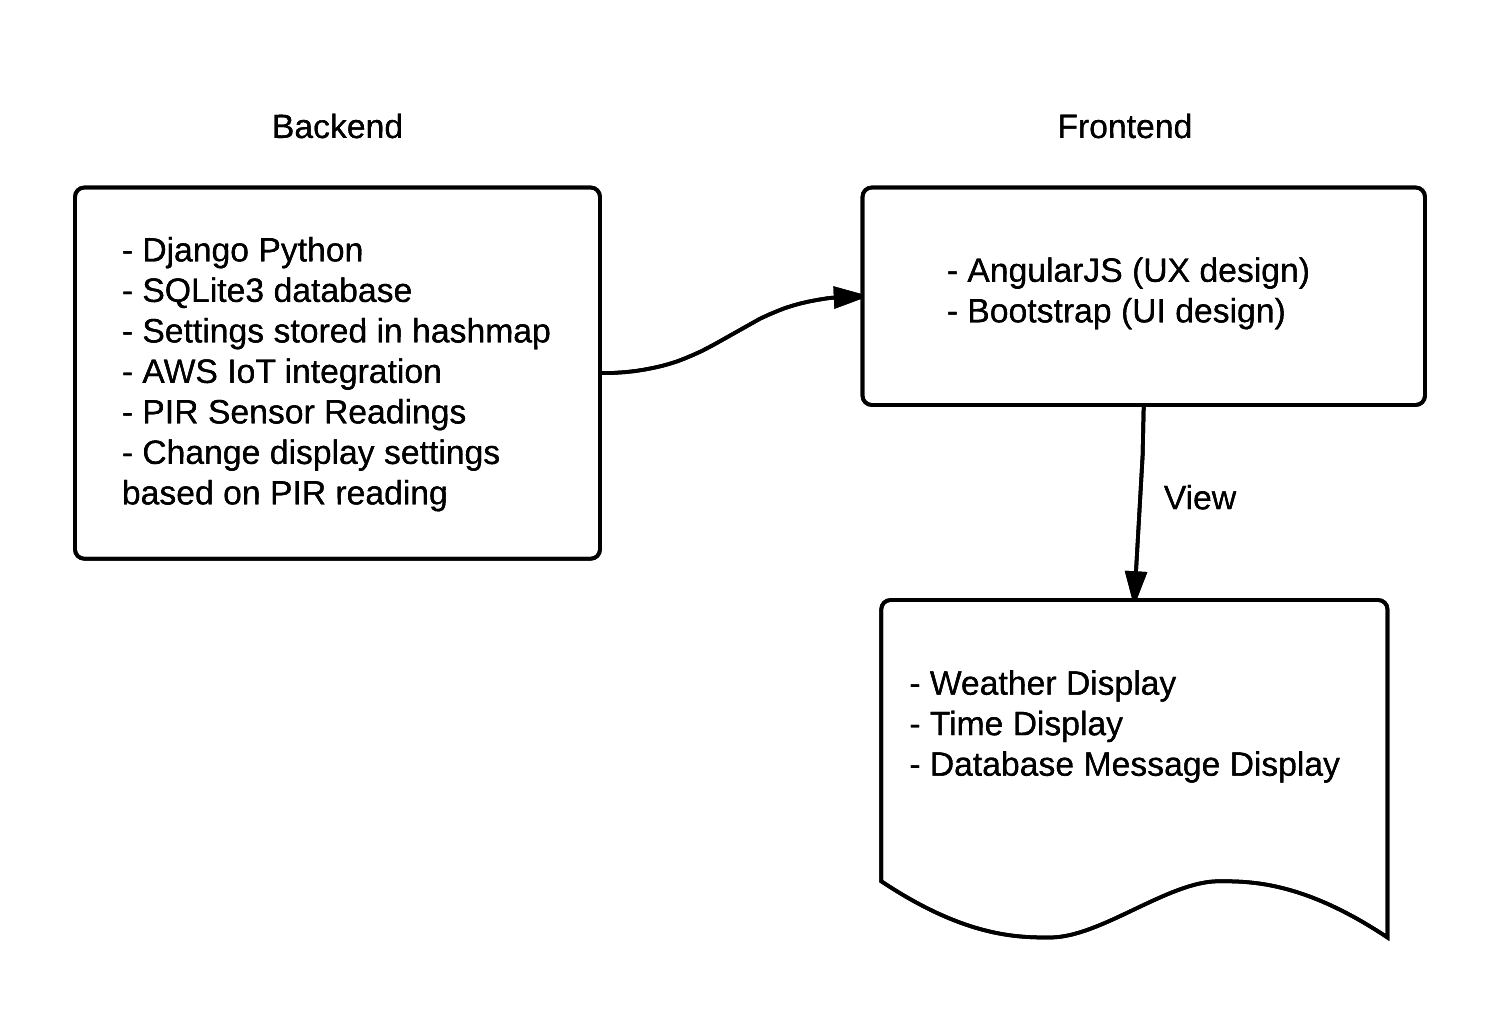
\includegraphics[width=2.5in]{images/DesignFlow.png}
  \caption{The design flow of the Magic Mirror software platform.}
  \label{fig:design}
\end{figure}

%angular and bootstrap frontend
%djago backend


\section{Analysis} 
%In the section of System, we focus on the big picture of the system and cover most issues that can be explained clearly. We often move heavy mathematical analysis of components and performance of the system into another section called Analysis or other appropriate names. 
The analysis section of this paper will involve 3 sections, Backend Code Review, Frontend Code Review, and Electronics.
Each section will talk about the methods used and all relevant details as to how the code was written or how the task was accomplished.

\subsection{Backend Code Review}
% talk about programming api here
The programming API of Magic Mirror is shown in Table \ref{tab:API}.
This API is leveraged by the client side of Magic Mirror for all of its settings and custom options.
The database for these settings is SQLite3 with a single table for all settings in the form of a hash map.
Each setting is simply a key value pair with no duplicates.
This pattern was used to create an easy integration between server and client side of Magic Mirror.

% API TABLE
\begin{table}[!ht]
\renewcommand{\arraystretch}{1.3}
\caption{Magic Mirror Backend API}
\label{tab:API}
\centering
\begin{tabular}{|c|c|L{4cm}|}
\hline
Type & Url & Description\\
\hline
\hline
GET & /magic\_mirror/settings/ & Returns all items contained in the database\\
\hline
POST & /magic\_mirror/settings/ & Adds a new item to the database as described by the payload\\
\hline
GET & /magic\_mirror/settings/\# & Returns a specific setting given by the ID \# in the url\\
\hline
PUT & /magic\_mirror/settings/\# & Updates a specific setting given by the ID \# in the url\\
\hline
DELETE & /magic\_mirror/settings/\# & Removes a specific setting given by the ID \# in the url\\
\hline
\end{tabular}
\end{table}

Additionally, The backend of Magic Mirror integrates with AWS IoT.
The PIR sensor status is communicated to AWS for statistical monitoring and security.
The Magic Mirror may also act as an intrusion detection system as the status of the mirror can be seen online through the dashboard.
This means that if a user wished to see if the Mirror was in use they need only check online.
More detail of this integration is shown in the Evaluation section of this paper.

\subsection{Frontend Code Review}
% talk about issues with getting bootstrap to play along with angular
% talk about having to write custom CSS
The frontend code of Magic Mirror was challenging due to its integration with both AngularJS and the Django backend framework.
By creating a wrapper for the API in AngularJS it was possible to bring all the needed functionality to the frontend.
The most important part was retrieving and organizing the settings so that the client could send requests to its other services such as weather.
Another challenge encountered while writing the frontend of Magic Mirror was making a UI which was both passive and useful.
The interface for the client must be passive as the only interaction that the user has with the device is the detection of the user.
Therefore, the interface must be useful but only at a glance.
This was challenging as it is simple to overload the user with textual information when so much is present.
As a design choice Magic Mirror has the room to add and remove options but by default only comes with the current weather and the current time as those two options are the most prevalent.

\subsection{Electronics}
% talk about issues with wiring the electronics here
As shown in Figure \ref{fig:elec}, the electronics for Magic Mirror are somewhat complex.
The bulk of the electronics were taken from a used LCD television which contained a logic board, power supply, and LCD panel.
Magic Mirror required the use of a Raspberry PI which is powered via a USB port at 5V and an HDMI port which was supplied by the television by default.
The 5V to power the PI was bridged off of the power supply for the television and wired to a sacrificial USB cord and an HDMI cable was run from the output of the Raspberry PI to the television.
All of the electronics were then mounted using hot glue to a corrugated plastic backing which was affixed to the picture frame.

% ELECTROINICS PICTURE
\begin{figure}[!ht]
  \centering
  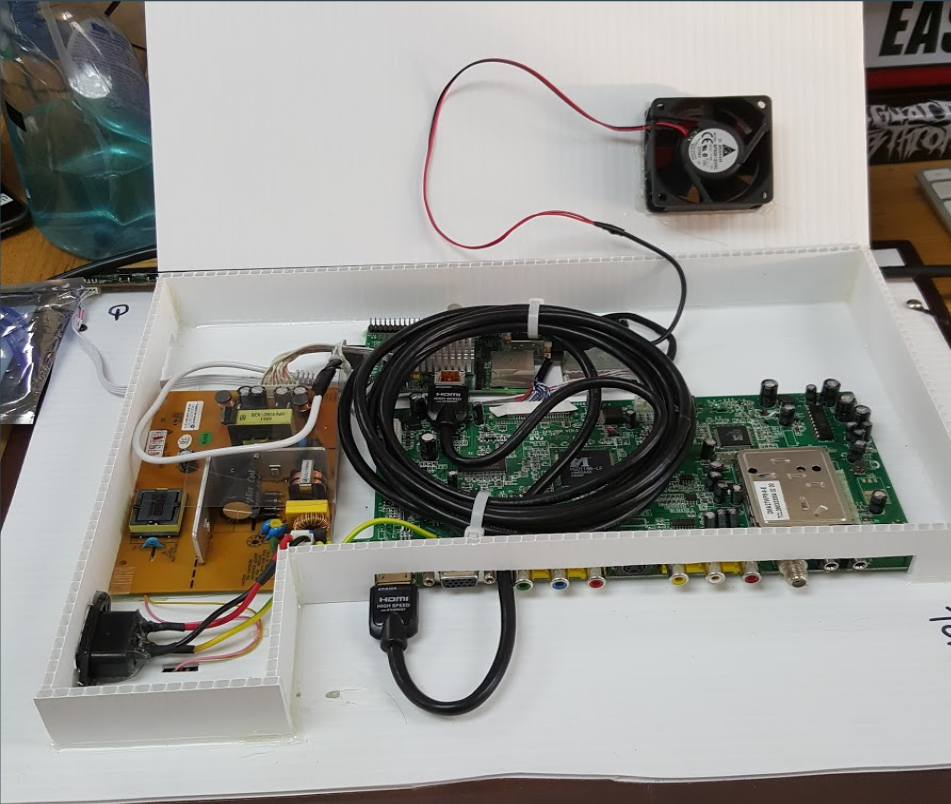
\includegraphics[width=2.5in]{images/Electronics.png}
  \caption{The completed electronics of the Magic Mirror}
  \label{fig:elec}
\end{figure}


\section{Evaluation}
%In this section, system performance is presented. How well does the system achieve its goal? Quantitative metrics should be used whenever necessary. Tables, figures with curves and charts are often used to show the performance such as the trend. To this end, 
  %whatever system students have developing, at least one week of data must be collected to show meaningful results. 
%For the alternative project on Edimax plug security, students should use Raspberry Pi to control the plug for at least one week and record the activities of turning on/off the plug with Raspberry Pi and other meaningful data.

\subsection{Motion Detection}
In keeping with the Security and Privacy aspects of this course, a portion of our testing was dedicated to exploring exactly what kind of information a device such as the Magic Mirror could collect if it were deployed in, for example, a user's home.
To that end, we collected motion detection data from the device's PIR sensor over the course of one week in the workspace of one of our group members.
Figures \ref{fig:chart26} and \ref{fig:chart29} show, by way of example, the data collected on April 26 and April 29, 2016, respectively.
The vertical axis shows the number of positive detections reported by the PIR sensor, and these are bucketed into twelve two-hour periods for each day's histogram.
Even these examples yield information as to when this individual spent the most time at his desk, at which the motion sensor was pointed.
\begin{figure}[!ht]
  \centering
  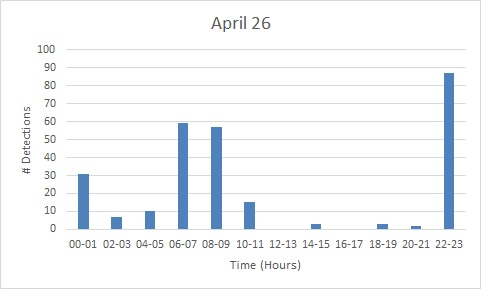
\includegraphics[width=2.75in]{images/Chart-April26.jpg}
  \caption{Histogram showing motion activity on April 26}
  \label{fig:chart26}
\end{figure}

\begin{figure}[!ht]
  \centering
  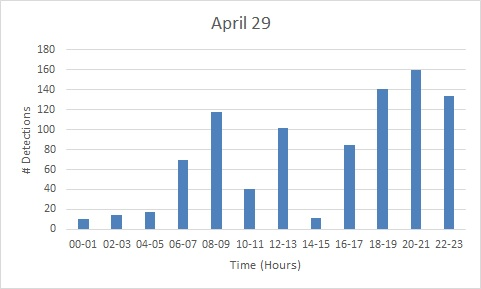
\includegraphics[width=2.75in]{images/Chart-April29.jpg}
  \caption{Histogram showing motion activity on April 29}
  \label{fig:chart29}
\end{figure}

By collecting this type of data over multiple days, we can begin to model the user's habits by calculating the average number of motion detections within a particular time interval over the course of the data collection period.
During our study spanning from April 24 to May 1 2016, we compiled a set of averages for each two-hour in the day. Figure \ref{fig:chartavg} plots these averages against their corresponding time intervals.
\begin{figure}[!ht]
  \centering
  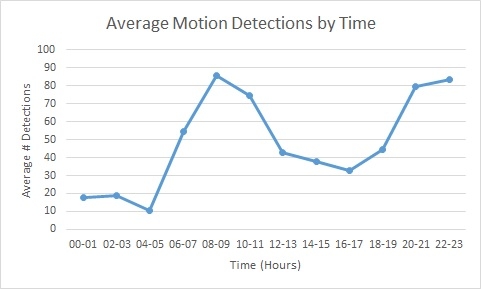
\includegraphics[width=2.75in]{images/Chart-averages.jpg}
  \caption{Average number of motion detections during each of 12 two-hour periods, from April 24 to May 1}
  \label{fig:chartavg}
\end{figure}

We can see in Figure \ref{fig:chartavg} that there are certain times when the user is relatively more likely to be moving within the field of view of the motion sensor.
In this case, 06 to 10 hours (6:00 AM to 10:00 AM) and 20 hours (8:00 PM) onward appear, on average, to be the times of greatest activity in this workspace.
Because the sensor senses at very short range, this places the individual within close proximity of the device itself.
As such, logging this data insecurely could compromise the privacy of the user by disclosing those times when the user is near the device, which could be used in conjunction with knowledge about the device's location to arrive at additional conclusions about that individual's daily routine.

\subsection{Mirror UI}
As the Magic Mirror's function is based largely on bringing aesthetically pleasing utility to a common wall fixture, our evaluation of the UI's success relies heavily upon the comments we received from those who observed the demonstration of the Magic Mirror during the final presentation session.
Those in attendance spoke favorably about the look and feel of the UI and the information it provides, with a few people noting that they would have use for a Magic Mirror of their own.
Figure \ref{fig:mirrorui} shows the Magic Mirror's informational UI for reference.
\begin{figure}[!ht]
  \centering
  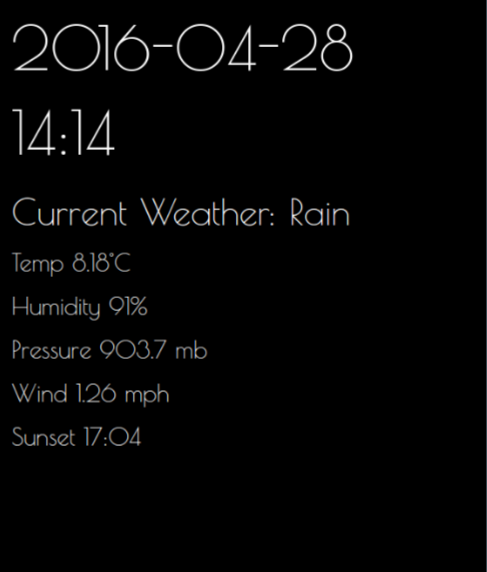
\includegraphics[width=2.75in]{images/mirror-ss.png}
  \caption{Screen capture of the Magic Mirror's information display UI}
  \label{fig:mirrorui}
\end{figure}


\section{Conclusion}
%In this section, the presented work is concluded. A brief introduction to the work is expected. Include the highlights of the work in conclusion. If necessary, future work can be discussed here.

% HARUN,
% talk about how using the PIR sensor as an intrusion detection method could be an extension of this application.
% conclude all thoughts contained above.
As stated, the main objective of the course was to implement an IOT device and connect it to the Amazon AWS, thereby understanding and analysing the security threats. And we implemented a Raspberry pie based smart mirror which displays the necessary informations to user when they stand infront of it. The PIR sensor attached along with the mirror detects the human presence thereby logging it into the Amazong Dynamo DB. By collecting the data over a period of time, in our case two weeks we can understand the behavioral pattern of the user. Some of the vital informations we analysed are the users daily routine for example the morning wake up time and thus future customisation for particular users is possible. By implementing the Smart mirror we analysed and understood the constraints one would face during the Iot development and various factors to be cared in respect to security.

% =====================================================  references section =======================================================
%References. At the end of the paper, there is always References. In the body of the paper, appropriate citations of references should be inserted into the right position, identifying related work. The list of references must not include references not cited in the paper. That is, references cannot be just listed without citations in the paper. Please use the reference and citation formatting in IEEE formatting template in this paper. 

% can use a bibliography generated by BibTeX as a .bbl file
% BibTeX documentation can be easily obtained at:
% http://mirror.ctan.org/biblio/bibtex/contrib/doc/
% The IEEEtran BibTeX style support page is at:
% http://www.michaelshell.org/tex/ieeetran/bibtex/
%\bibliographystyle{IEEEtran}
% argument is your BibTeX string definitions and bibliography database(s)
%\bibliography{IEEEabrv,../bib/paper}
%
% <OR> manually copy in the resultant .bbl file
% set second argument of \begin to the number of references
% (used to reserve space for the reference number labels box)
\begin{thebibliography}{1}

%\bibitem{IEEEhowto:kopka}
%H.~Kopka and P.~W. Daly, \emph{A Guide to \LaTeX}, 3rd~ed.\hskip 1em plus
 % 0.5em minus 0.4em\relax Harlow, England: Addison-Wesley, 1999.
  "Xonay Labs | Michael Teeuw." Xonay Labs | Michael Teeuw. N.p., n.d. Web. 05 May 2016.
  
  Michaelteeuw. "Magic Mirror: Part I - The Idea & The Mirror." Xonay Labs. N.p., n.d. Web. 05 May 2016.
 
  "A Magic Mirror Powered by a Raspberry Pi. Best Christmas Present I've Ever Put Together. Detailed Tutorial in Comments." Imgur. N.p., n.d. Web. 05 May 2016.


\end{thebibliography}

\end{document}


